\documentclass[conference]{IEEEtran}
\usepackage{graphicx,booktabs,amsmath}
\usepackage[hidelinks]{hyperref}
\title{Local Traffic Speed Forecasting on METR-LA\\A Reproducible Phase 1 Benchmark}
\author{\IEEEauthorblockN{Pankaj Baid, Ashutosh Singh, Shreya Suman\\Narendra Singh, Ranvendra Pratap Singh}}
\begin{document}
\maketitle
\begin{abstract}
We present a reproducible Phase 1 benchmark for local traffic-speed forecasting on METR-LA. The preserved dataset contains 34,272 five-minute timestamps from 207 sensors. A shared causal pipeline generates 32 features, uses chronological training, validation and test partitions, and leaves unavailable targets unimputed. Persistence, historical averages, Random Forest and two XGBoost configurations are evaluated at 5, 15, 30 and 60 minutes. The 36-feature XGBoost extension with training-history averages obtains test MAEs of 2.312, 2.844, 3.275 and 3.688, reducing persistence MAE by 17.8\% to 31.5\%. Independent prediction-row scoring adds all-model temporal slices, sensor-level forecast-error maps and paired day-block uncertainty. The 32-feature learner comparison is distinguished from the history-feature extension. Unknown speed units, timezone and freeway identities are retained as limitations. These results establish a traceable local baseline for a future graph-model experiment; graph superiority is not evaluated here.
\end{abstract}
\begin{IEEEkeywords}Traffic forecasting, METR-LA, Random Forest, XGBoost, chronological evaluation, spatial errors.\end{IEEEkeywords}
\section{Introduction}
Traffic-speed forecasting provides a measurable foundation for congestion analysis. A useful first stage is to determine how far a sensor's own recent measurements and recurring temporal patterns can predict its future speed. This question should be answered before attributing an improvement to network structure or adding simulation and control objectives.

Phase 1 therefore compares local forecasts under a common data contract. Each forecast row describes one sensor at one prediction origin. Models may be fitted to pooled examples from all sensors, but an individual input contains only the target sensor's own history and allowed temporal variables. Neighboring measurements, coordinates, adjacency-derived features and sensor identity are excluded from the shared 32-feature input.

The contribution is a reproducible benchmark with shared quality rules, timestamp boundaries and target masks. Five configurations are scored on identical held-out rows, followed by temporal, sensor and regional error analysis.

\section{Related Work And Scope}
The METR-LA dataset is associated with the traffic-forecasting evaluation in DCRNN [1]. Its spatiotemporal framework uses a directed-graph formulation, whereas this phase deliberately restricts predictive inputs to local observations. Our custom target offsets, sample eligibility and feature design should not be treated as an exact reproduction of the published DCRNN experiment.

Random Forest combines randomized trees [2], while XGBoost provides efficient tree boosting [3]. Their regression configurations have different loss preferences. To limit selection bias [4], this evaluation preserves fitted booster artifacts and fixed RF settings. Graph attention [5] is a candidate for a future spatial experiment.

\section{Data And Chronological Protocol}
\subsection{Raw data quality and provenance}
The source speed table contains 34,272 ordered five-minute timestamps and 207 sensors, covering March 1 through June 27, 2012 on the stored clock. There are no duplicate or absent timestamps and no NaN, infinite or negative raw readings. The 575,302 exact-zero cells represent 8.109\% of measurements and are conservatively treated as unavailable benchmark readings. These include 2,148 all-sensor-zero timestamps in 97 contiguous blocks; their physical causes are not established. Raw bytes are preserved and checked against the acquisition manifest.

The speed table's sensor order matches the available 207 by 207 adjacency inventory and location metadata. This alignment supports later graph work, but graph assets do not enter the Phase 1 predictive features. The inspected metadata does not independently verify physical speed units or timezone. We therefore use source speed units and the stored clock throughout, including the peak definitions.

\begin{table}[t]
\caption{Shared chronological partitions}
\centering\footnotesize
\begin{tabular}{lrrr}
\toprule
Partition & Grid times & Origins & Rows\\
\midrule
Train & 23,990 & 23,967 & 4,961,169\\
Validation & 3,427 & 3,416 & 707,112\\
Test & 6,855 & 6,844 & 1,416,708\\
\bottomrule
\end{tabular}
\end{table}
\subsection{Sample boundaries and unavailable observations}
The timestamp grid is partitioned chronologically into 70\% training, 10\% validation and 20\% test observations. For origin t, history spans t-11 through t; target offsets are 1, 3, 6 and 12 five-minute steps. All four targets must belong to the same partition. Earlier observed history can come from a preceding partition because it is already available at the prediction origin. No time shuffling or model-specific split is permitted.

Input zeros and other invalid readings are masked and forward filled. Leading gaps use the corresponding sensor's training median. Training medians, historical averages and reference speeds are fitted on the training interval only. No backfill or future interpolation is used, and target values remain raw. Long outages may therefore produce stale repeated inputs; two missingness features preserve evidence of this condition. The test valid-target counts are 1,245,052, 1,245,040, 1,245,022 and 1,244,986 at the four horizons.

\section{Features Models And Common Metrics}
\subsection{Shared features and model configurations}
The 32 shared features comprise 12 current/past speed lags; eight causal rolling mean, standard-deviation, minimum and maximum statistics; three speed-change terms; seven cyclic/calendar/peak variables; and two missingness indicators. Every rolling window ends at the forecast origin. RF ablations use 12 lags (A), 19 lags plus temporal features (B), 27 lags plus temporal and rolling features (C), and all 32 features (D).

Persistence predicts the forward-filled current speed at every horizon. Historical average predicts the sensor's training-only mean for the target weekday and five-minute slot, excluding unavailable observations and using its training mean when a lookup cell is absent. RF uses 100 trees, maximum depth 15, bootstrap max\_samples 0.1 and seed 42. The same settings are held fixed for all 16 horizon/feature-group fits.

Each XGBoost model predicts the residual from current speed with an absolute-error objective. The preserved settings use histogram trees, depth 8, learning rate 0.1, minimum child weight 50, row and column subsampling 0.8, and seed 42. Training used validation early stopping. Completion re-evaluates the eight saved boosters rather than changing their fitted parameters.

The history-augmented booster adds expected speed at target and origin times, their difference, and the current deviation from expected speed. Training lookups exclude the row's own relevant reading. Its 36 local features provide additional information; RF 32 versus XGBoost 32 remains the direct learner comparison.

\subsection{Aligned evaluation and error definitions}
The evaluation first verifies unique origin/sensor keys, exact row order, target arrays, target-validity flags and stored-clock temporal flags across prediction files and the shared dataset. Every model must supply finite predictions. Invalid targets are excluded identically; a failed prediction on a valid target raises an error rather than silently reducing the scored sample. An empty slice is represented as unscored, not zero error.

For N finite positive observed targets, MAE and RMSE use the usual absolute and squared differences. MAPE is 100 times the average absolute error divided by max(y, 0.00001). The explicit denominator floor retains positive near-zero targets in all three metrics. Scores are computed from saved prediction values, with counts reported for each horizon and group.

\begin{equation}\mathrm{MAE}=\frac{1}{N}\sum_i |y_i-\hat y_i|\end{equation}
\begin{equation}\mathrm{RMSE}=\sqrt{\frac{1}{N}\sum_i (y_i-\hat y_i)^2}\end{equation}
\begin{equation}\mathrm{MAPE}=\frac{100}{N}\sum_i\frac{|y_i-\hat y_i|}{\max(y_i,10^{-5})}\end{equation}
\section{Held Out Forecasting Results}
\begin{table}[t]
\caption{Test mae}
\centering\footnotesize
\begin{tabular}{lrrrr}
\toprule
Model & 5 min & 15 min & 30 min & 60 min\\
\midrule
Persistence & 2.814 & 3.499 & 4.206 & 5.380\\
Historical average & 4.188 & 4.188 & 4.188 & 4.189\\
RF 32 & 2.452 & 3.167 & 3.871 & 4.854\\
XGBoost 32 & 2.362 & 2.970 & 3.564 & 4.393\\
XGBoost + HA 36 & 2.312 & 2.844 & 3.275 & 3.688\\
\bottomrule
\end{tabular}
\end{table}
\begin{table}[t]
\caption{Test rmse}
\centering\footnotesize
\begin{tabular}{lrrrr}
\toprule
Model & 5 min & 15 min & 30 min & 60 min\\
\midrule
Persistence & 4.627 & 6.418 & 8.052 & 10.344\\
Historical average & 7.855 & 7.855 & 7.855 & 7.855\\
RF 32 & 4.156 & 5.763 & 7.002 & 8.410\\
XGBoost 32 & 4.151 & 5.806 & 7.129 & 8.720\\
XGBoost + HA 36 & 4.065 & 5.540 & 6.546 & 7.470\\
\bottomrule
\end{tabular}
\end{table}
\begin{table}[t]
\caption{Test mape percent}
\centering\footnotesize
\begin{tabular}{lrrrr}
\toprule
Model & 5 min & 15 min & 30 min & 60 min\\
\midrule
Persistence & 6.49 & 8.61 & 10.86 & 14.53\\
Historical average & 13.04 & 13.04 & 13.04 & 13.04\\
RF 32 & 6.02 & 8.56 & 11.10 & 14.48\\
XGBoost 32 & 5.76 & 7.92 & 10.27 & 13.74\\
XGBoost + HA 36 & 5.66 & 7.63 & 9.49 & 11.34\\
\bottomrule
\end{tabular}
\end{table}
XGBoost plus HA achieves the lowest MAE among the evaluated configurations at every horizon. Its MAE reduction relative to persistence grows from 17.8\% at 5 minutes to 31.5\% at 60 minutes. Historical-average MAE is approximately horizon independent because it queries a recurring target-time profile; small differences arise from the eligible target rows.

The local information restriction matters for interpretation. At 60 minutes, plain XGBoost has MAE 4.393, compared with 4.189 for historical average. Adding the historical features yields 3.688. This demonstrates a useful feature extension on this split; it does not isolate a graph effect or show that a local model family has reached a universal limit.

MAE and RMSE can rank the learners differently. Plain XGBoost optimizes absolute error, whereas RF uses a squared-error splitting criterion. RF has lower RMSE than plain XGBoost at the longer horizons even when its MAE is higher. This is an observed tradeoff between the fitted configurations and objectives, so all three metrics are retained instead of selecting only the metric favorable to one model.

\begin{figure}[t]
\centering
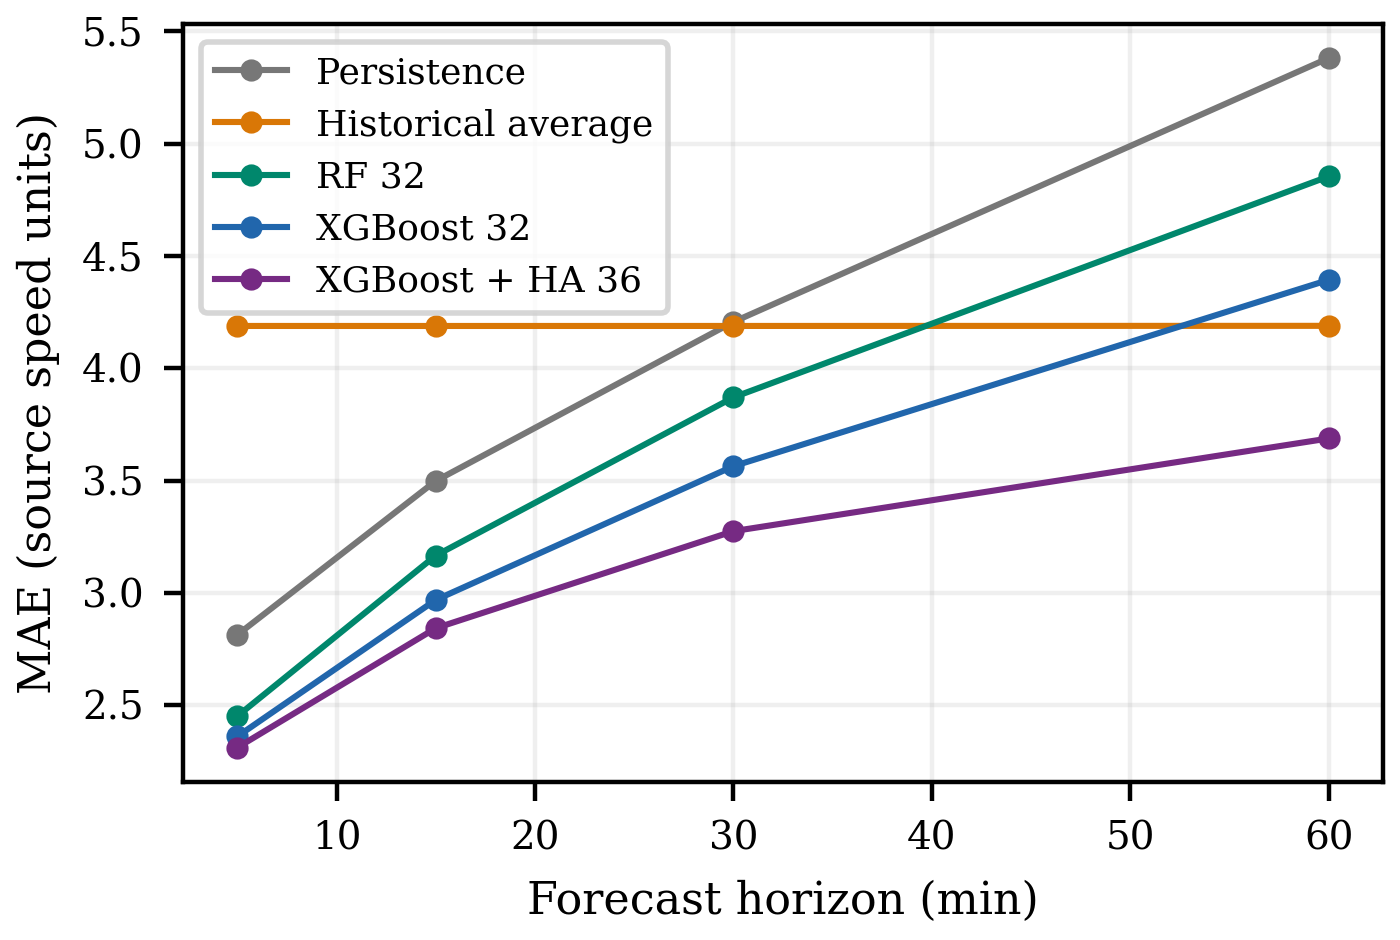
\includegraphics[width=\columnwidth]{figures/horizon_mae.png}
\caption{Test MAE across forecast horizons. The history-augmented booster uses 36 features; RF and plain XGBoost share 32.}
\end{figure}
\subsection{Temporal slices and feature ablations}
Peak groups are weekday origin hours [07:00,10:00) and [16:00,19:00) on the stored clock. Their union is combined peak; off peak includes all other origins and weekends. Targets may fall after an origin-period boundary.

For 15-minute XGBoost plus HA forecasts, off-peak, morning and evening MAEs are 2.555, 3.469 and 4.484. Evening-origin MAE is 75.5\% higher than off-peak MAE. RF uses the same slices and target masks. These stored-clock differences are descriptive, with no event-level causal attribution.

\begin{figure}[t]
\centering
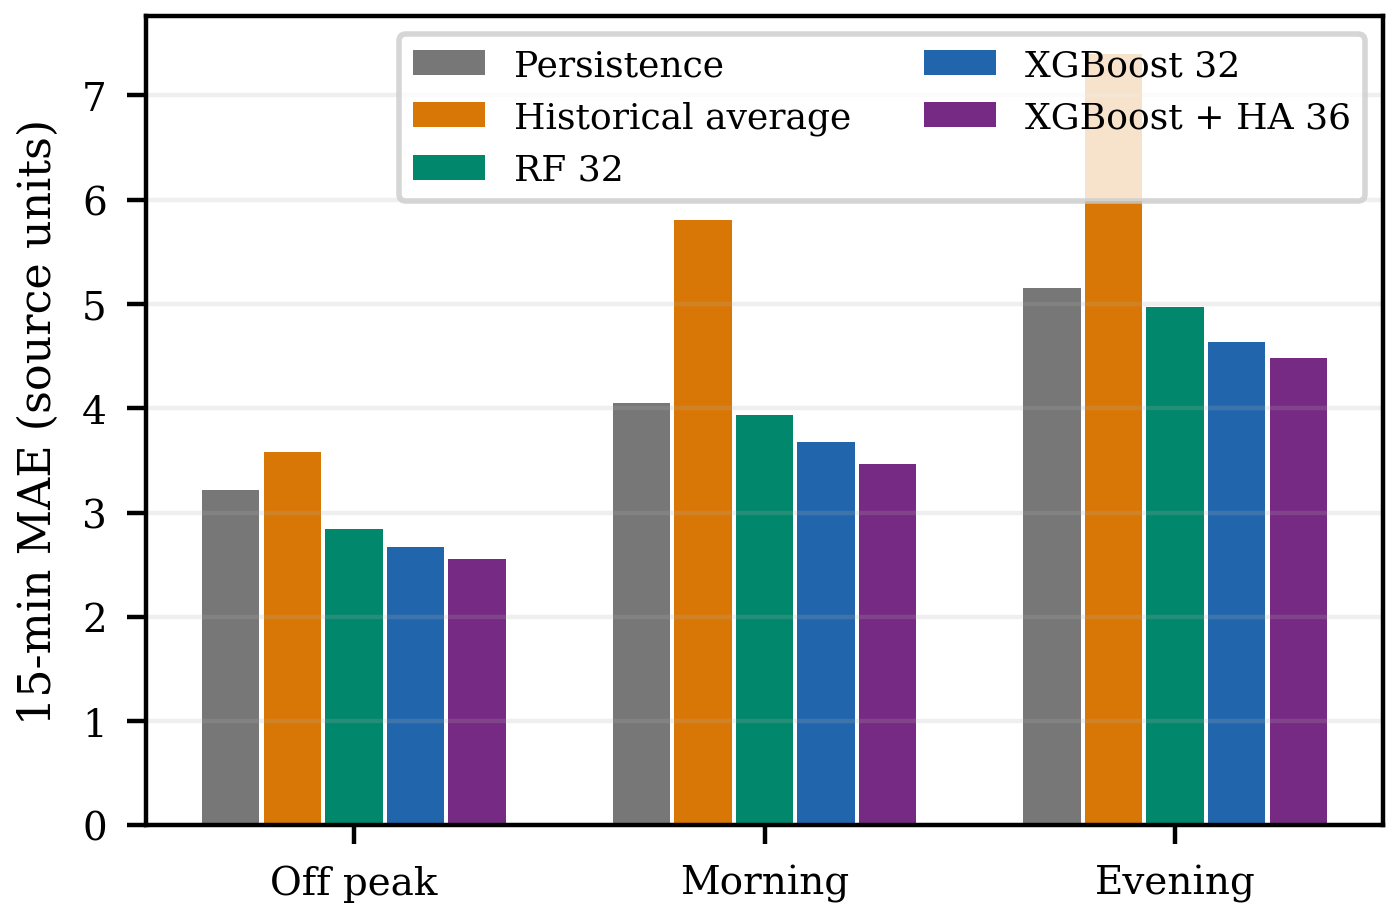
\includegraphics[width=\columnwidth]{figures/temporal_mae.png}
\caption{The 15-minute temporal comparison includes all five configurations and identical valid targets within each origin-period slice.}
\end{figure}
The RF ablations isolate the value of the declared feature groups under identical fixed fitting settings. Temporal and rolling features are particularly useful relative to the lag-only configuration at longer horizons. Adding every remaining feature need not improve every score: the 27-feature group can slightly outperform the full 32-feature group. Complete ablation metrics, fit times and feature definitions accompany the machine-readable evidence.

\section{Spatial Errors And Paired Uncertainty}
\subsection{Observed and predicted congestion diagnostics}
Spatial evaluation joins verified sensor coordinates to per-sensor forecast errors on valid held-out targets. It compares observed and predicted means, MAE, RMSE, MAPE and observation counts, rather than using observed speed variability as a forecast-error surrogate. Morning and evening maps are generated separately for RF and XGBoost plus HA. Geographic aggregates sum errors and counts before division, avoiding unweighted means of sensor scores with unequal data availability.

Coordinates are verified, but named freeways and traffic direction are not. Regions are labelled coordinate bins. Each sensor's training 85th percentile provides an operational speed reference. Descriptive peak summaries slice raw observation times and use valid-count weights; forecast maps slice origins and score future targets.

For a reproducible congestion-frequency diagnostic, observed and predicted speeds below 60\% of the sensor reference are counted on identical valid targets. Thresholds are fitted on training observations only. This proxy enables predicted-versus-observed congestion maps without inventing incident or queue labels. Its calibration against verified congestion events remains outside the available evidence.

\begin{figure}[t]
\centering
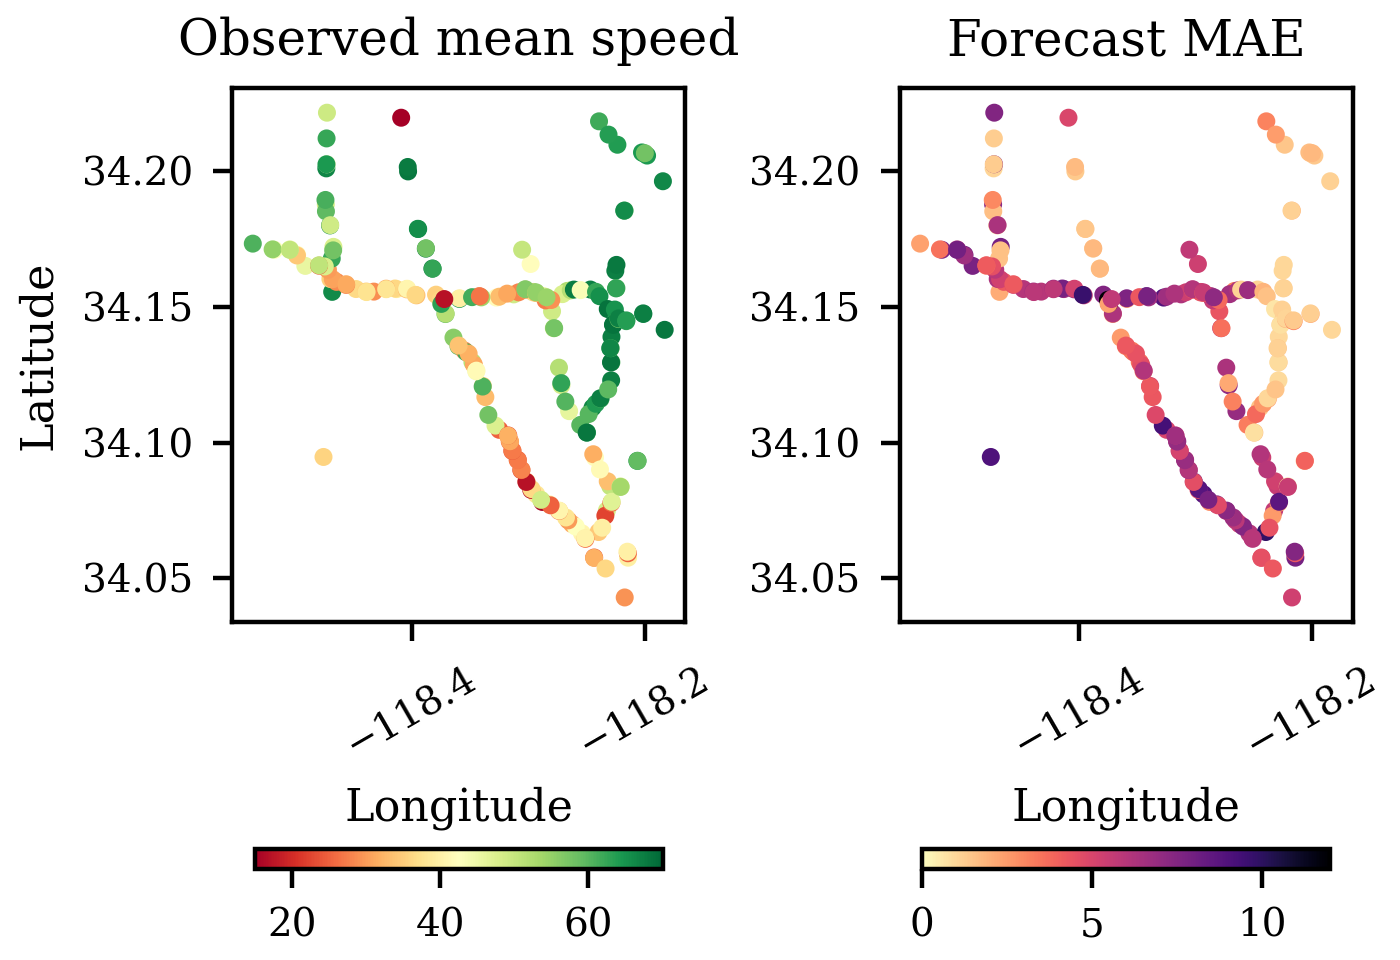
\includegraphics[width=\columnwidth]{figures/spatial_errors.png}
\caption{XGBoost plus HA 15-minute evening-origin predictions: observed mean speed and actual forecast MAE by sensor. Both panels use the same valid test targets and source speed units.}
\end{figure}
\subsection{Paired blocks of stored calendar days}
Forecast errors are correlated across nearby times and sensors. We therefore avoid treating approximately 1.245 million target rows as independent samples for an uncertainty calculation. Instead, all observed targets and sensors within each stored calendar day are retained together. We draw 2,000 paired circular moving-block bootstrap samples, each assembled from blocks of two consecutive days, using seed 42.

Each resampled absolute-error difference is divided by the common valid-target count. Positive values favor the candidate. The 2.5\% and 97.5\% percentiles form conditional intervals for this test period; they do not adjust for model selection or establish validity in other cities or seasons.

\begin{table}[t]
\caption{Paired 60 minute mae reduction}
\centering\footnotesize
\begin{tabular}{lrr}
\toprule
Baseline vs candidate & Reduction & 95\% interval\\
\midrule
Persistence vs XGBoost + HA 36 & 1.693 & 1.466 to 1.894\\
RF 32 vs XGBoost 32 & 0.460 & 0.427 to 0.505\\
XGBoost 32 vs XGBoost + HA 36 & 0.706 & 0.580 to 0.827\\
\bottomrule
\end{tabular}
\end{table}
A retrospective time-series example is selected from the highest-MAE sensor for the 60-minute history-augmented booster and centered on its largest valid absolute error. This diagnostic selection is disclosed and is never used for model tuning. The resulting traces illustrate local forecast deviations; they do not identify a verified incident, infer a queue propagation speed or establish causality.

\begin{figure}[t]
\centering
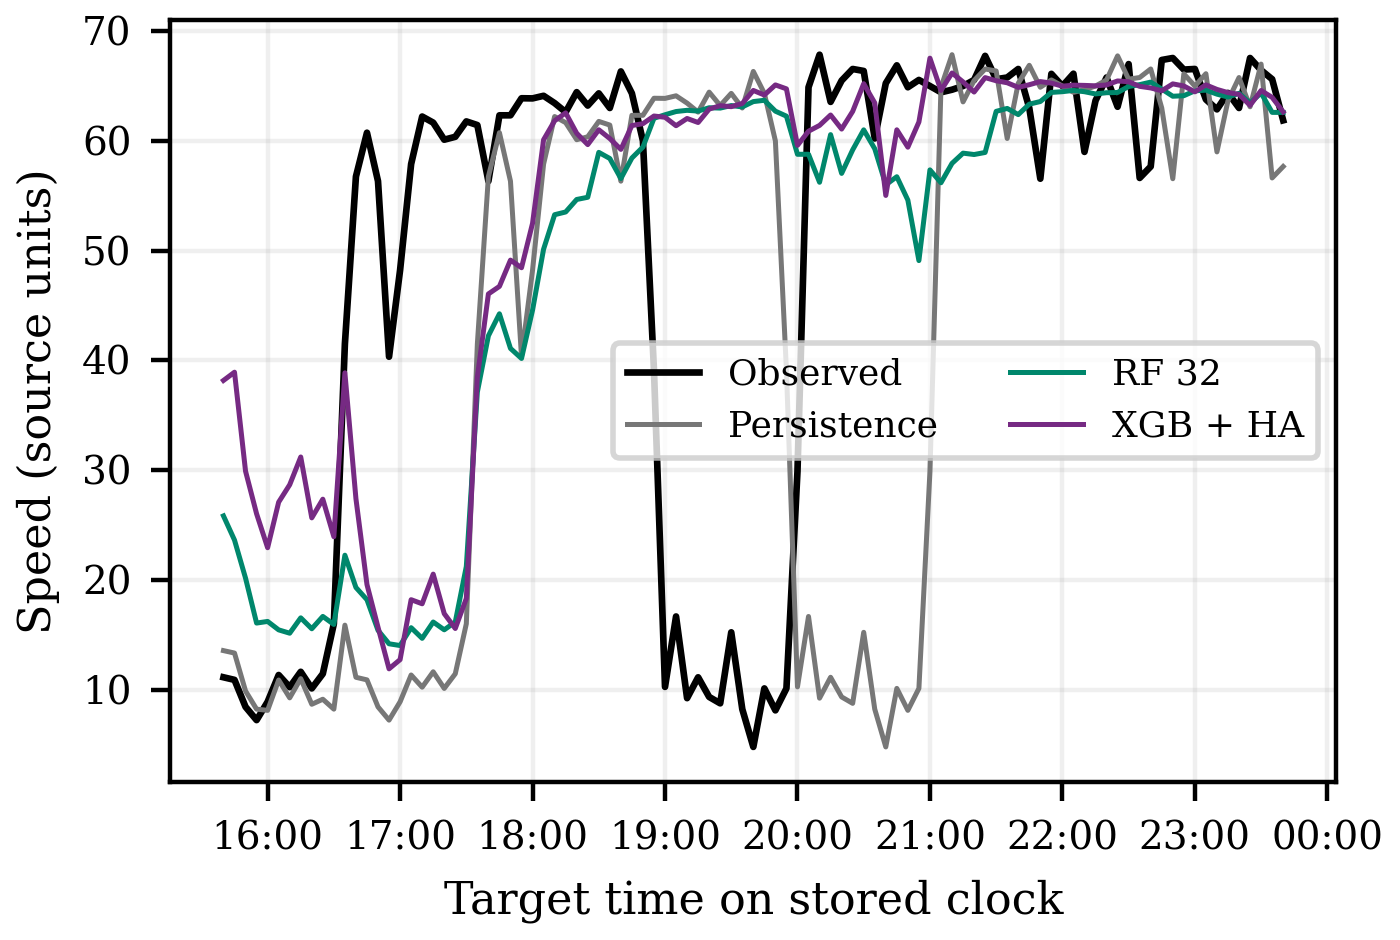
\includegraphics[width=\columnwidth]{figures/forecast_example.png}
\caption{Retrospective 60-minute forecast example for sensor 717468. Lines are positioned at target time. The example is selected for error inspection after evaluation.}
\end{figure}
\section{Reproducibility And Limitations}
The repository provides features, predictions, model artifacts, common scoring and executed notebooks. SHA-256 manifests record raw data, model, dataset and forecast inputs with runtime versions. Per-sensor error sums reconstruct pooled MAE, and valid-target counts are checked against the raw-derived dataset.

RF is regenerated with fixed settings; frozen boosters are re-scored with official XGBoost 3.4.1. An optional numeric-JSON reader preserves tree order and best iteration. It matches both a direct scalar walk and the official runtime exactly on 96 deterministic validation rows for each of the eight boosters.

The lower valid-target fraction in test limits coverage of outage conditions, and forward-filled inputs can remain stale for hours. Evidence covers one chronological split and one seed per configuration. Unverified units, clock, road identity and proxy congestion labels constrain physical and causal interpretation.

A future graph comparison should preserve the splits and masks, include strong temporal comparators and repeated seeds, and test the value of neighboring observations. No graph model or traffic-signal control is evaluated here.

\section{Conclusion}
The benchmark integrates local forecasts, all-model temporal slices, sensor errors, congestion maps and paired uncertainty. The history-augmented XGBoost reaches 3.688 MAE at 60 minutes, while the shared-feature RF/XGBoost comparison preserves a clear distinction between learner and feature effects. The result is a traceable baseline for subsequent experiments rather than a claim of demonstrated graph superiority.

\begin{thebibliography}{00}
\bibitem{ref1} Y. Li, R. Yu, C. Shahabi, and Y. Liu, "Diffusion convolutional recurrent neural network: Data-driven traffic forecasting," in Proc. Int. Conf. Learning Representations, 2018. arXiv:1707.01926.
\bibitem{ref2} L. Breiman, "Random forests," Machine Learning, vol. 45, pp. 5-32, 2001, doi: 10.1023/A:1010933404324.
\bibitem{ref3} T. Chen and C. Guestrin, "XGBoost: A scalable tree boosting system," in Proc. 22nd ACM SIGKDD Int. Conf. Knowledge Discovery and Data Mining, 2016, pp. 785-794, doi: 10.1145/2939672.2939785.
\bibitem{ref4} G. C. Cawley and N. L. C. Talbot, "On over-fitting in model selection and subsequent selection bias in performance evaluation," Journal of Machine Learning Research, vol. 11, pp. 2079-2107, 2010.
\bibitem{ref5} P. Velickovic, G. Cucurull, A. Casanova, A. Romero, P. Lio, and Y. Bengio, "Graph attention networks," in Proc. Int. Conf. Learning Representations, 2018. arXiv:1710.10903.
\end{thebibliography}
\end{document}
